\begin{pastexam}[label={px:ntu-109-ee-ds-19}]{臺大電機所 109 學年度（B）第 19 題}
（複選；每題 4 分，每答錯一個選項倒扣 0.8 分至該題 0 分止）

Consider the AVL tree in Fig.1.
\begin{enumerate}[label=(\Alph*)]
\item In Fig.1, after inserting the key 66, then the parent of key 66 is key 61.
\item In Fig.1, after inserting the key 99, then the key 95 has two children.
\item In Fig.1, after inserting the key 30, then the parent of key 30 is key 35.
\item In Fig.1, after deleting the key 75, then the key 87 has two children.
\item In Fig.1, after deleting the key 1, then the parent of key 23 is key 13.
\end{enumerate}

\begin{center}
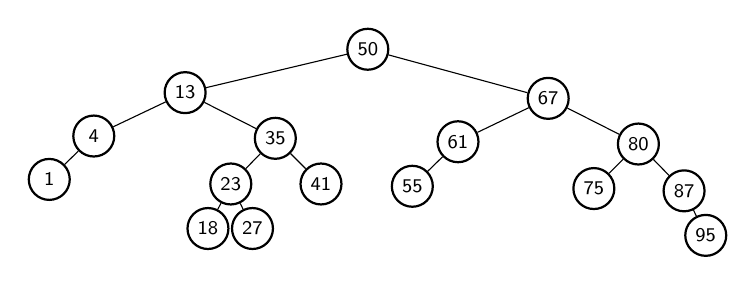
\begin{tikzpicture}[x=1.45cm,y=1.45cm,v/.style={draw,thick,circle,minimum size=5.2mm,inner sep=0pt,font=\scriptsize\sffamily}]
  \foreach \n/\x/\y in {50/7.06/4.12,13/5.46/4.50,67/8.64/4.55,4/4.66/4.88,35/6.25/4.90,61/7.85/4.93,80/9.43/4.95,
                        1/4.27/5.26,23/5.86/5.30,41/6.65/5.30,55/7.45/5.32,75/9.04/5.34,87/9.83/5.36,18/5.66/5.69,27/6.05/5.69,95/10.02/5.75} {
    \node[v] (\n) at (\x,-\y) {\n};
  }
  \foreach \a/\b in {50/13,50/67,13/4,13/35,4/1,35/23,35/41,23/18,23/27,67/61,67/80,61/55,80/75,80/87,87/95} { \draw (\a) -- (\b); }
\end{tikzpicture}\\ Fig.1 AVL tree
\end{center}
\end{pastexam}

\begin{pastsoln}
答案：(A)、(B)、(C)、(D)。

先標出 Fig.1 各節點的高度（葉節點算 $0$）：$18, 27, 41, 1, 55, 75, 95$ 是 $0$；$23, 4, 61, 87$ 是 $1$；
$35, 80$ 是 $2$；$13, 67$ 是 $3$；$50$ 是 $4$。 每個節點左右高度差都不超過 $1$，是合法的 AVL 樹。 每個
選項都從 Fig.1 原本的樹開始做。 插入、刪除後從改動的位置往根走，找第一個左右高度差變成 $2$ 的節點，
依 LL、LR、RR、RL 四種情形旋轉（資結書第~10.2.3~、10.2.6~節）。

\textbf{(A) 插入 66：對。} 路徑 $50 \to 67 \to 61$，$66 > 61$，接在 $61$ 的右邊。 $61$ 變成左右各一個
子節點，高度仍是 $1$，往上都沒有改變，不用旋轉。 $66$ 的父節點是 $61$。

\textbf{(B) 插入 99：對。} 路徑 $50 \to 67 \to 80 \to 87 \to 95$，接在 $95$ 的右邊。 $95$ 高度變 $1$；
$87$ 的左子樹是空的（高度記成 $-1$）、右子樹高度 $1$，差 $2$，不平衡。 新鍵在 $87$ 的右子節點的右邊，
是 RR，對 $87$ 做一次左旋轉：$95$ 上來，左子節點 $87$、右子節點 $99$。 旋轉後這棵子樹高度回到 $1$，和
插入前一樣，上面不用再處理。 $95$ 有兩個子節點。

\textbf{(C) 插入 30：對。} 路徑 $50 \to 13 \to 35 \to 23 \to 27$，接在 $27$ 的右邊。 往上更新高度：$27$
變 $1$，$23$ 變 $2$（左 $18$ 高 $0$、右 $27$ 高 $1$，差 $1$，還平衡）；$35$ 的左子樹 $23$ 高 $2$、右子樹
$41$ 高 $0$，差 $2$，不平衡。 新鍵在 $35$ 的左子節點 $23$ 的\textbf{右}子樹裡，是 LR，做雙旋轉：$27$
升到 $35$ 的位置，$23$ 成為它的左子節點，$35$ 成為它的右子節點；$27$ 原本的右子樹（$30$）接到 $35$
的左邊。
\begin{center}
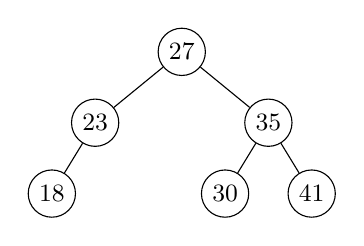
\begin{tikzpicture}[level distance=9mm,every node/.style={circle,draw,minimum size=6mm,inner sep=0pt,font=\small},
  level 1/.style={sibling distance=22mm},level 2/.style={sibling distance=11mm}]
\node {27} child {node {23} child {node {18}} child[missing]} child {node {35} child {node {30}} child {node {41}}};
\end{tikzpicture}
\end{center}
這棵子樹高度 $2$，和插入前的 $35$ 一樣，上面不用再處理。 $30$ 的父節點是 $35$。

\textbf{(D) 刪除 75：對。} $75$ 是葉節點，直接拿掉。 $80$ 的左子樹變空（高度 $-1$），右子樹 $87$ 高 $1$，
差 $2$。 右子節點 $87$ 的左邊空、右邊有 $95$，偏右，是 RR，對 $80$ 做左旋轉：$87$ 上來，左子節點 $80$、
右子節點 $95$。 這棵子樹高度從 $2$ 變 $1$，往上檢查：$67$ 左 $61$ 高 $1$、右 $87$ 高 $1$，平衡；$50$
左高 $3$、右高 $2$，平衡。 $87$ 有兩個子節點。

\textbf{(E) 刪除 1：錯。} $1$ 是葉節點，拿掉後 $4$ 的高度變 $0$。 $13$ 的左子樹 $4$ 高 $0$、右子樹 $35$
高 $2$，差 $2$。 右子節點 $35$ 的左子樹 $23$ 高 $1$、右子樹 $41$ 高 $0$，偏左，是 RL，做雙旋轉：$23$
升到 $13$ 的位置，$13$ 成為它的左子節點（帶著 $4$，並接上 $23$ 原本的左子樹 $18$），$35$ 成為它的右
子節點（接上 $23$ 原本的右子樹 $27$）。
\begin{center}
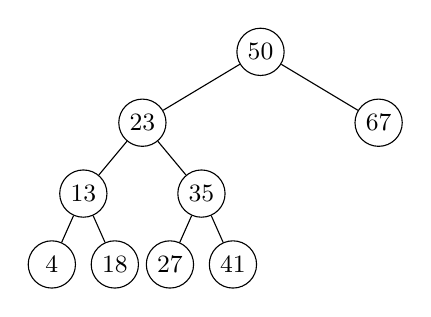
\begin{tikzpicture}[level distance=9mm,every node/.style={circle,draw,minimum size=6mm,inner sep=0pt,font=\small},
  level 1/.style={sibling distance=30mm},level 2/.style={sibling distance=15mm},level 3/.style={sibling distance=8mm}]
\node {50} child {node {23} child {node {13} child {node {4}} child {node {18}}} child {node {35} child {node {27}} child {node {41}}}}
  child {node {67}};
\end{tikzpicture}
\end{center}
（右邊 $67$ 的子樹沒有變，省略。） 子樹高度變 $2$；$50$ 的左高 $2$、右高 $3$，仍平衡。 $23$ 的父節點
是 $50$，不是 $13$。 注意 RL 的情形要用雙旋轉；只對 $13$ 做一次左旋轉會讓 $35$ 上來、$23$ 接到 $13$
右邊，結果仍然不平衡，那樣才會得到「$23$ 的父節點是 $13$」。
\end{pastsoln}
